% % % % % % % % % % % % % % % % % % % % % % % % % % % % % % % % % % % % % % % % % % % %
%                                                                                     %
% Short Sectioned Assignment LaTeX Template Version 1.0 (5/5/12)                      %
% This template has been downloaded from: http://www.LaTeXTemplates.com               %
%                                                                                     %
% Original author:  Frits Wenneker (http://www.howtotex.com)                          %
%                                                                                     %
% Modified by: Fco Javier Sueza Rodríguez (fcosueza@disroot.org)                      %
%                                                                                     %
% Changes:                                                                            %
%	    - Custom Chapters, Sections and Subsections (titlesec package)                %
%           - Document type scrbook (oneside)                                         %
%           - Use babel-lang-spanish package and marvosym                             %
%           - Use hyperref, enumitem, tcolorbox and glossaries packages               %
%           - Use Time New Roman (mathptmx), Helvetic and Courier fonts               %
%                                                                                     %
% License: CC BY-NC-SA 3.0 (http://creativecommons.org/licenses/by-nc-sa/3.0/)        %
%                                                                                     %
% % % % % % % % % % % % % % % % % % % % % % % % % % % % % % % % % % % % % % % % % % % %

%-----------------------------------------------%
%	              Packages                  %
%-----------------------------------------------%

\documentclass[paper=a4, fontsize=11pt, oneside]{scrbook}

% ---- Text Input/Output ----- %

\usepackage[T1]{fontenc}
\usepackage[utf8]{inputenc}
\usepackage{mathptmx}
\usepackage[scaled=.92]{helvet}
\usepackage{courier}
\usepackage[indent=12pt]{parskip}

\usepackage{geometry}
\geometry{verbose,tmargin=3cm,bmargin=3cm,lmargin=2.6cm,rmargin=2.6cm}

% ---- Language ----- %

\usepackage[spanish]{babel}
\usepackage{marvosym}

% ---- Another packages ---- %

\usepackage{amsmath,amsfonts,amsthm}
\usepackage{graphics,graphicx}
\usepackage{titlesec}
\usepackage{fancyhdr}
\usepackage{tcolorbox}
\usepackage{hyperref}
\usepackage{enumitem}
\usepackage[automake]{glossaries}

%--------------------------------------------------------------------%
%                      Customizing Document                          %
%--------------------------------------------------------------------%


% ----------- Custom Chapters, Sections and Subsections -------------- %

\titleformat{\chapter}[display]
			{\bfseries\Huge}
			{Tema \ \thechapter} {0.5ex}
			{\vspace{1ex}\centering}

\titleformat{\section}[hang]
			{\bfseries\Large}
			{\thesection}{0.5em}{}

\titleformat{\subsection}[hang]
			{\bfseries\large}
			{\thesubsection}{0.5em}{}

\titleformat{\subsubsection}[hang]
			{\bfseries\large}
			{\thesubsubsection}{0.5em}{}

\hypersetup{
    colorlinks=true,
    linkcolor=black,
    urlcolor=magenta
}

% ------------------- Custom heaaders and footers ------------------- %

\pagestyle{fancyplain}

\fancyhead[]{}
\fancyfoot[L]{}
\fancyfoot[C]{}
\fancyfoot[R]{\thepage}

\renewcommand{\headrulewidth}{0pt} % Remove header underlines
\renewcommand{\footrulewidth}{0pt} % Remove footer underlines

\setlength{\headheight}{13.6pt} % Customize the height of the header

% --------- Numbering equations, figures and tables ----------------- %

\numberwithin{equation}{section} % Number equations within sections
\numberwithin{figure}{section} % Number figures within sections
\numberwithin{table}{section} % Number tables within sections

% ------------------------ New Commands ----------------------------- %

\newcommand{\horrule}[1]{\rule{\linewidth}{#1}} % Create horizontal rule command


%----------------------------------------------------------------------------------------
%	TÍTULO Y DATOS DEL ALUMNO
%----------------------------------------------------------------------------------------

\title{
\vspace{10ex}
\normalfont \normalsize
\Huge \textbf{Tarea 4: Realización de Consultas}
}
\author{Francisco Javier Sueza Rodríguez}
\date{\normalsize\today}

%----------------------------------------------------------------------------------------
%                                     DOCUMENTO
%----------------------------------------------------------------------------------------
\begin{document}

\maketitle

\thispagestyle{empty}

\vspace{68ex}

\begin{center}
    \begin{tabular}{l l}
        \textbf{Centro}: & IES Aguadulce \\
        \textbf{Ciclo Formativo}: & Desarrollo Aplicaciones Web (Distancia)\\
        \textbf{Asignatura}: & Bases de Datos\\
        \textbf{Tema}: & Tema 4 -  Realización de Consultas\\
    \end{tabular}
\end{center}

\newpage

\tableofcontents

\newpage

\listoffigures

\newpage

\section{Caso Práctico}
Alejandro es el gerente de la empresa CUIDA TU CUERPO. Esta empresa se fundó en 2021 y su principal línea de negocio es el entrenamiento personal de los clientes, para ello cuenta con una serie de fisioterapeutas y profesores de pilates. Para ello ha recurrido a la empresa de Carla para que le puedan diseñar la base de datos que pueda almacenar toda la información necesaria para su gestión.

Carla se lo ha comentado al resto del equipo y todos están de acuerdo en realizar la base datos. Por lo tanto Ana va a realizar la base de datos. Como miembro del equipo de trabajo de Ana, estás trabajando directamente con la base de datos. El análisis y diseño está ya realizado, así como la implementación en MySQL, ahora se han cargado una serie de datos de prueba para probar las sentencias de consultas que el representante de las distintas asociaciones nos ha pedido entre los requisitos que desean.

Tu tarea es realizar dichas sentencias SQL para MySQL probándolas con los datos que se han cargado de prueba para comprobar el resultado de cada consulta y verificar si es correcto o no.

Como compañeros de Ana, debemos ayudarle para realizar las consultas propuestas

\section{Actividades}
Para poder acceder a información de una Base de Datos, ésta debe estar creada y debe contener registros previamente. Por tanto, lo primero que debes realizar es descargar el script que contiene las tablas y datos que encontrarás en el apartado 2.- ``Información de interés'', además de seguir todos los consejos y recomendaciones para elaborar esta tarea que en dicho apartado se explican.

Lo que realmente se pide en la tarea es que ayudes a Ana redactando las sentencias SQL que ejecuten cada una de las siguientes consultas correctamente en MySQL.

\subsection{Aparatado A}
Elabora las \textbf{sentencias SQL} para realizar las siguientes consultas:

\begin{enumerate}
    \item Obtener un listado de todos los clientes.
    \item Obtener el nombre y stock de los productos que tengan menos de 50 unidades de stock ordenados de menor a mayor.
    \item Obtener los nombres y apellidos de los profesionales que trabajan en el horario de tarde (desde las 15:00) y cuál es su horario.
    \item Obtener una lista con los clientes que estén dados de baja y tengan un descuento mayor de 40.
\end{enumerate}

\subsection{Aparatado B}
Elabora las \textbf{sentencias SQL} para realizar las siguientes consultas:

\begin{enumerate}
    \setcounter{enumi}{4}
    \item Obtener la fecha y hora de la cita, el nombre y apellidos del cliente y el número de trabajador del fisioterapeuta para todas las citas a domicilio, ordenadas por fecha y hora de forma ascendente.
    \item Obtener el producto que más cuesta y el que menos cuesta, indicando su valor.
    \item Obtener un listado donde se muestre por cada uno de los estados en los que puede estar un profesor de pilates, la cantidad total de profesores que existen por cada uno de ellos.
    \item Obtener por cada mes que haya tenido al menos una cita (con el formato de nombre y no de número ej. Noviembre), la cantidad de citas realizadas en 2022 ordenadas por número de citas de mayor a menor.
    \item Obtener un histórico de todas las citas del cliente ‘27256987J’ dónde se pueda ver el numero trabajador del fisioterapeuta que le trató, la fecha y el precio de las citas.
    \item Obtener un listado de todos los fisioterapeutas que han dado citas fuera de su horario, mostrando en qué fecha la dieron en formato DD/MM/AAAA.
    \item Obtener un listado con la fecha de la última cita que se dio y el nombre y apellidos del cliente que asistió.
    \item Obtener un listado con el nombre y apellidos de cada profesor de pilates que no estén ni despedidos ni ausentes y también la cantidad de clases que han impartido ordenados de mayor a menor por la cantidad de clases.
    \item Obtener por cada producto cuantas unidades se han vendido, mostrar también los productos que no hayan tenido ninguna venta.
    \item Obtener los nombres, apellidos y teléfonos de los fisioterapeutas que trabajen menos de 5 horas al día y estén trabajando actualmente.
    \item Obtener un listado de clases de pilates que hayan sido impartidas por más de un profesor, indicando el nombre de la sala, el día, la hora de la clase y número de profesores.
    \item Obtener un listado con el precio medio de las citas de 2022 por cada fisioterapeuta que esté trabajando, mostrar número de fisio y el precio medio.
\end{enumerate}

\subsection{Apartado C}

\begin{enumerate}
    \setcounter{enumi}{16}
    \item Obtener un listado con el nombre de la sala y el nombre completo del profesor de pilates junto al número de veces que dicho profesor ha utilizado cada una de las salas donde al menos haya impartido clase el mismo profesor en la misma sala 2 o más veces.
    \item Obtener el DNI y nombre de cada cliente junto a la cantidad total que lleva gastada en fisioterapeutas, siempre y cuando esa cantidad total sea superior a la media de todas las citas.
\end{enumerate}

\section{Soluciones}
En esta sección vamos a poner todas las soluciones a las consultas que se nos piden, acompañadas cada una de una captura de pantalla con el resultado obtenido en \textbf{MySQL Workbench}.

\begin{figure}[H]
    \begin{tcolorbox}[sharp corners, colback=blue!30, colframe=white!20]
        \normalsize
\textbf{NOTA IMPORTANTE} \\


Esta tarea se ha realizado en Linux, el cual distingue entre mayúsculas y minúsculas, por lo que para que el script proporcionado con la tarea haya realizado la creación de tablas y adición de datos correctamente, se ha habilitado la opción \textbf{lower\_case\_table\_names}, que básicamente convierte el nombre de todas la tablas a minúsculas, por lo que en caso de utilizar las consultas en un sistema Linux esta opción deberá estar también habilitada en el servidor MySQL. También puede modificarse el script proporcionado y poner el nombre de las tablas en minúscula en las sentencias \textbf{CREATE DATABASE}.
    \end{tcolorbox}
\end{figure}

\subsection{Apartado A}

\begin{enumerate}
    \item Solución:

    \begin{figure}[h]
        \begin{tcolorbox}[sharp corners, colback=yellow!30, colframe=white!20]
            \scriptsize
            \begin{verbatim}


          SELECT * FROM cliente;  \end{verbatim}
        \end{tcolorbox}
    \end{figure}

    \begin{figure}[H]
        \centering
        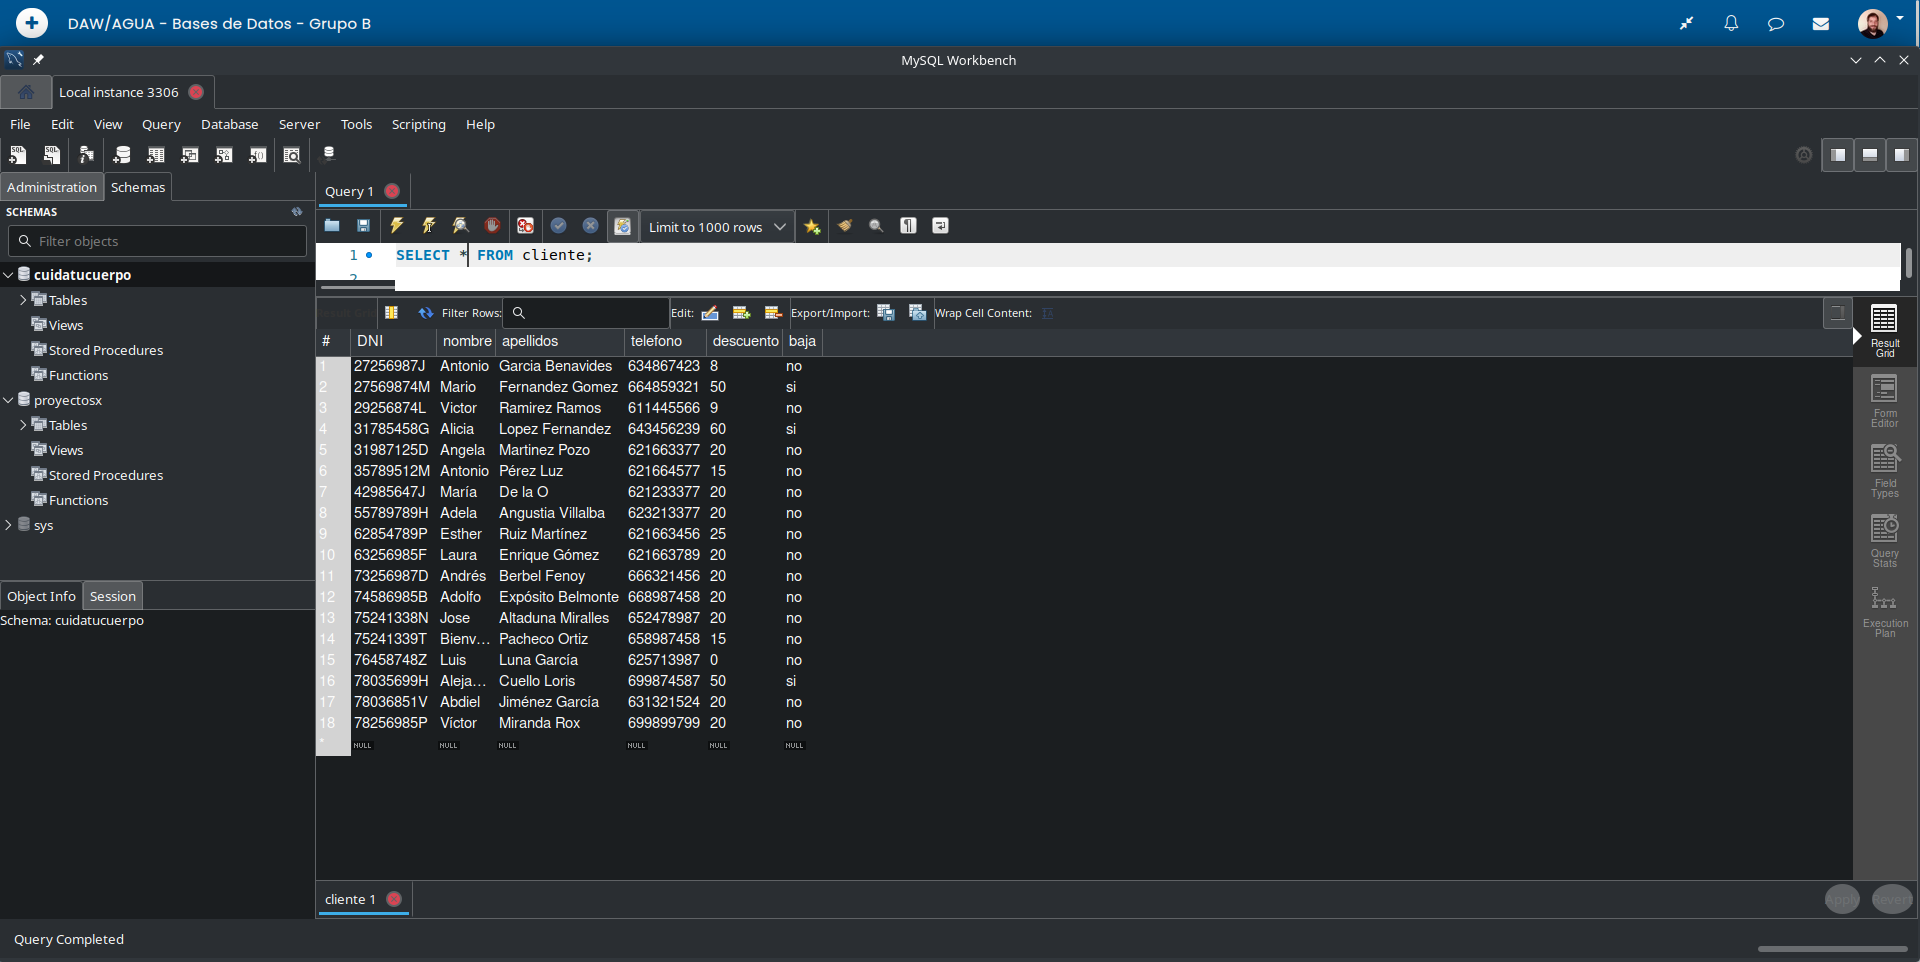
\includegraphics[scale=0.28]{resultado-consulta-1.png}
        \caption{Resultado Consulta nº 1}
    \end{figure}

    \item Solución:

    \begin{figure}[h]
        \begin{tcolorbox}[sharp corners, colback=yellow!30, colframe=white!20]
            \scriptsize
            \begin{verbatim}


         SELECT nombre, stock FROM productos WHERE stock<50 ORDER BY stock ASC;
            \end{verbatim}
        \end{tcolorbox}
    \end{figure}

    \begin{figure}[H]
        \centering
        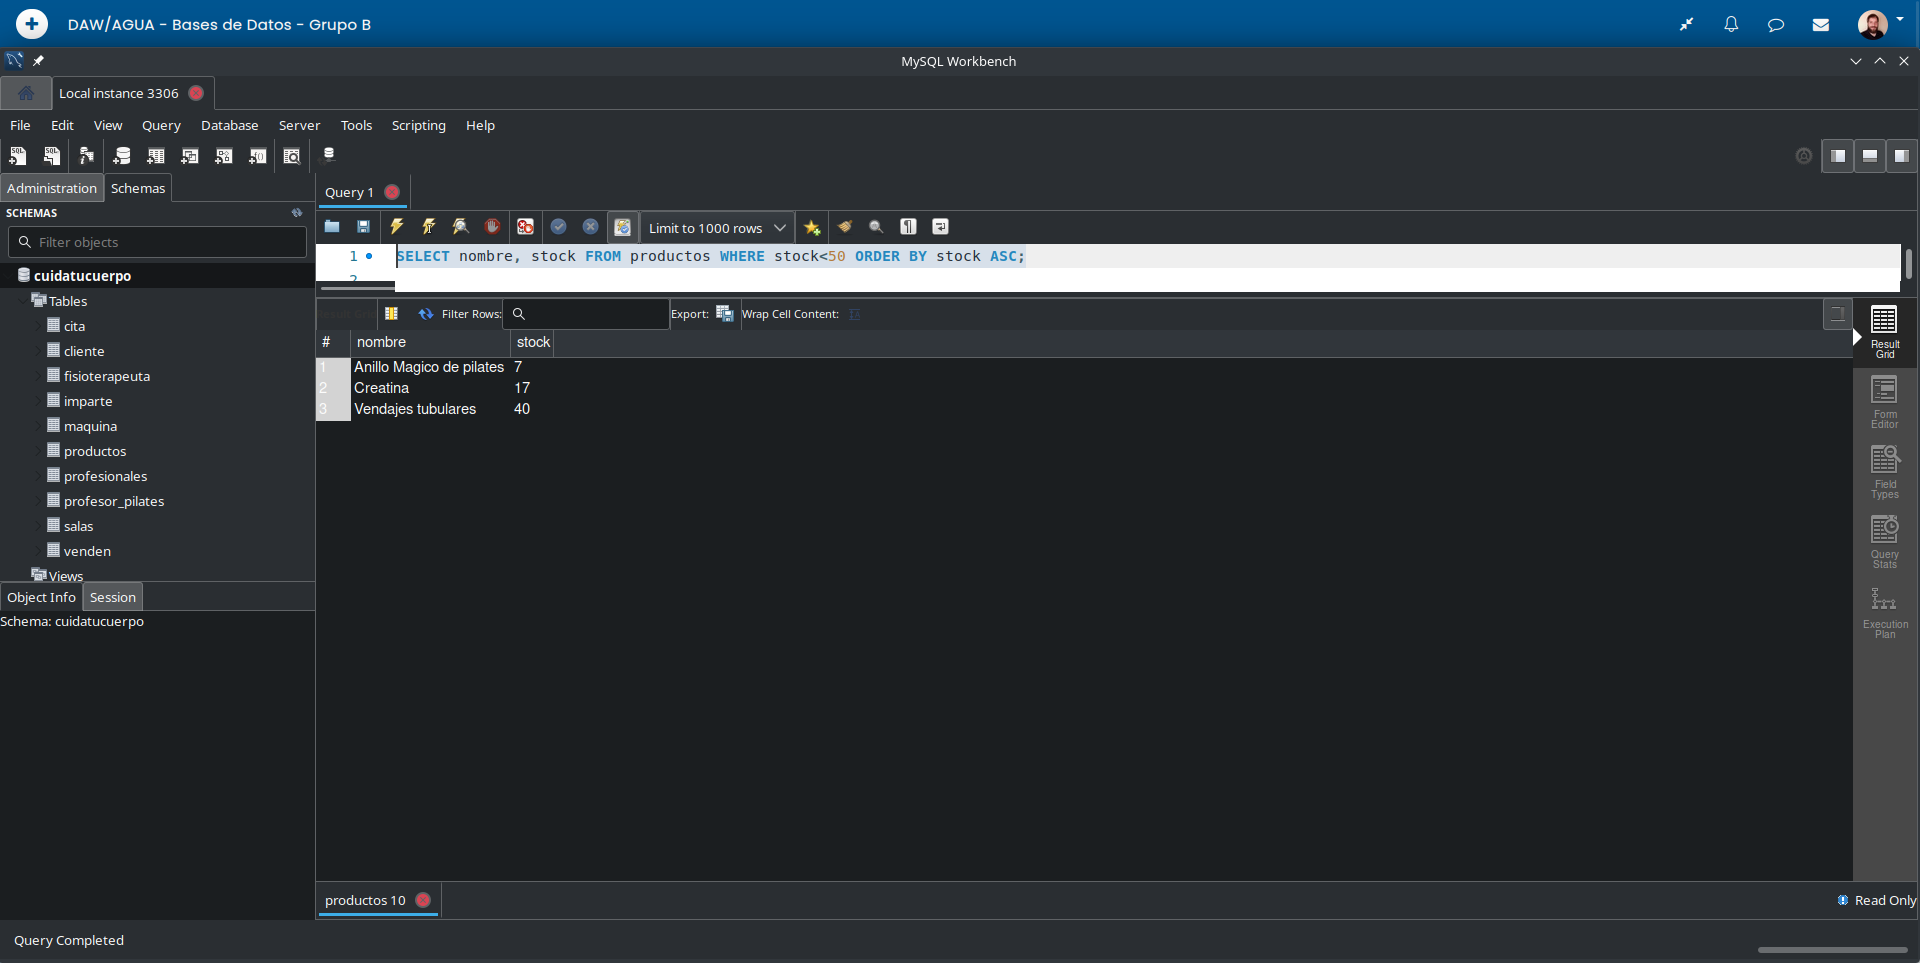
\includegraphics[scale=0.28]{resultado-consulta-2.png}
        \caption{Resultado Consulta nº 2}
    \end{figure}

    \item Solución:

      \begin{figure}[H]
        \begin{tcolorbox}[sharp corners, colback=yellow!30, colframe=white!20]
            \scriptsize
            \begin{verbatim}


          SELECT nombre, apellidos, CONCAT(hora_inicio, " - ", hora_fin) AS horario
          FROM profesionales
          WHERE hora_inicio > "15:00";
            \end{verbatim}
        \end{tcolorbox}
    \end{figure}

    \begin{figure}[H]
        \centering
        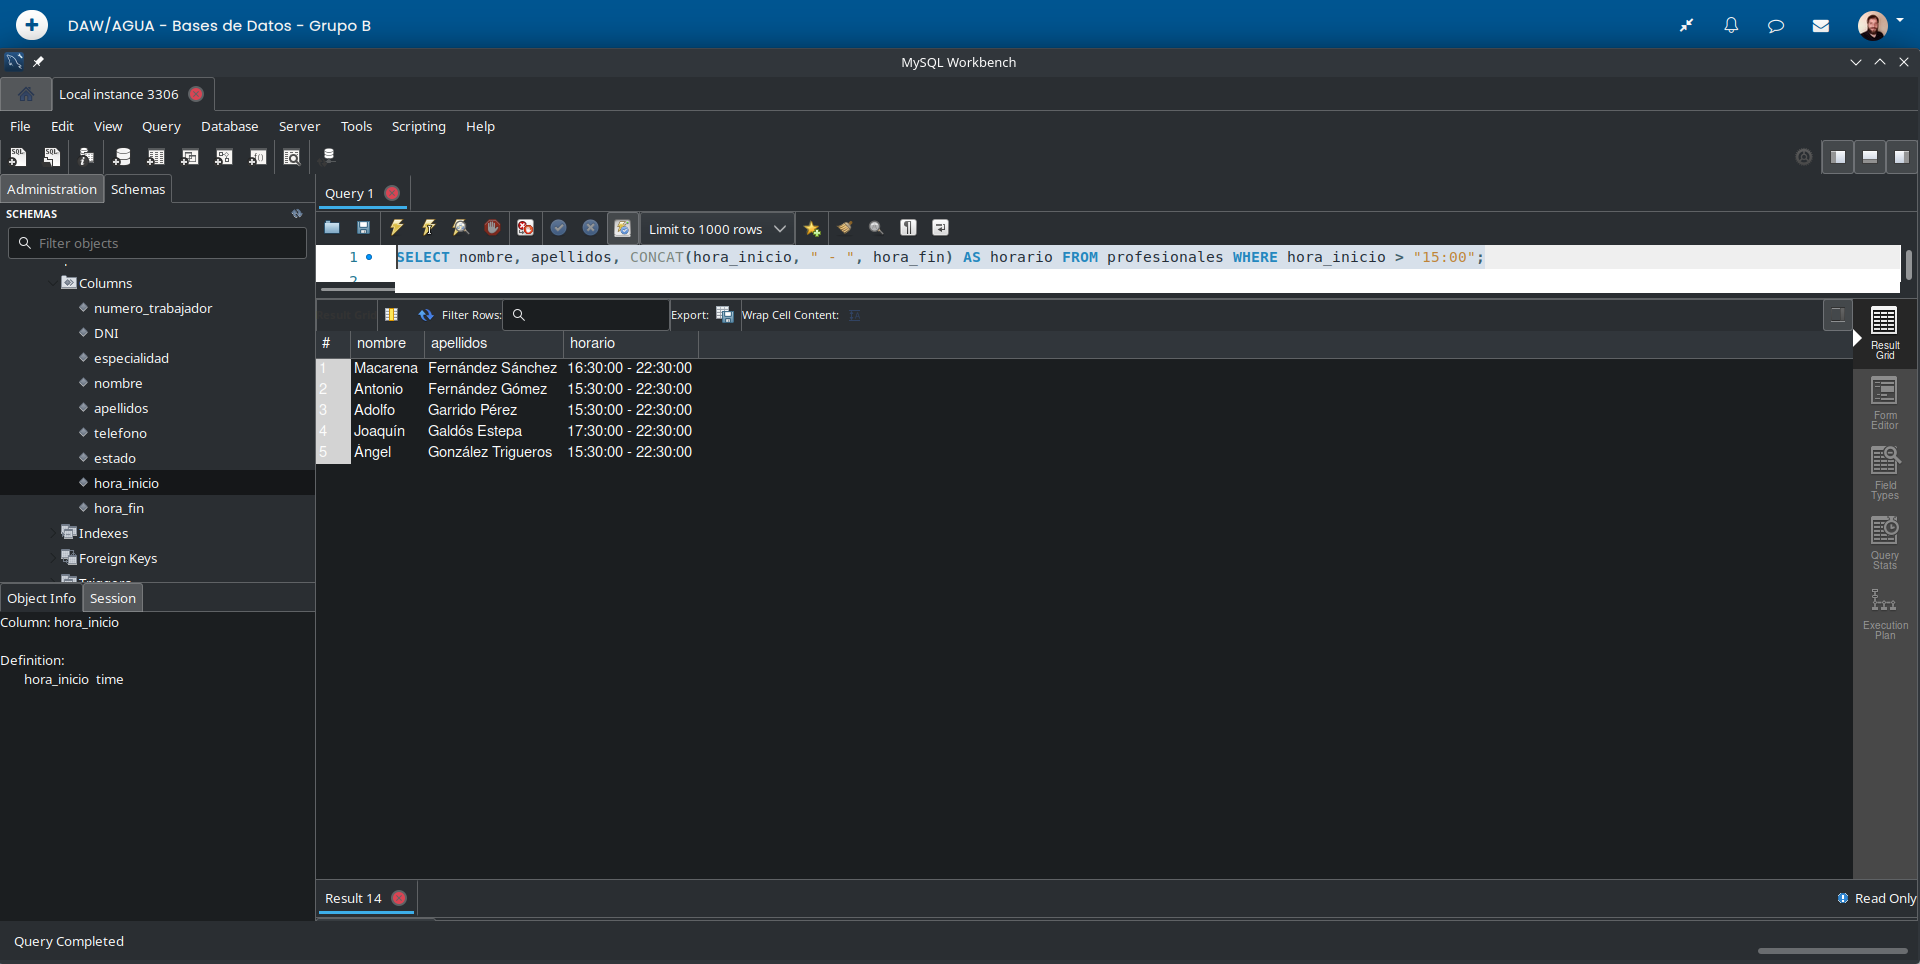
\includegraphics[scale=0.28]{resultado-consulta-3.png}
        \caption{Resultado Consulta nº 3}
    \end{figure}

    \item Solución:

    \begin{figure}[H]
        \begin{tcolorbox}[sharp corners, colback=yellow!30, colframe=white!20]
            \scriptsize
            \begin{verbatim}


        SELECT * FROM cliente WHERE baja = "si" AND descuento > 40;
            \end{verbatim}
        \end{tcolorbox}
    \end{figure}

    \begin{figure}[H]
        \centering
        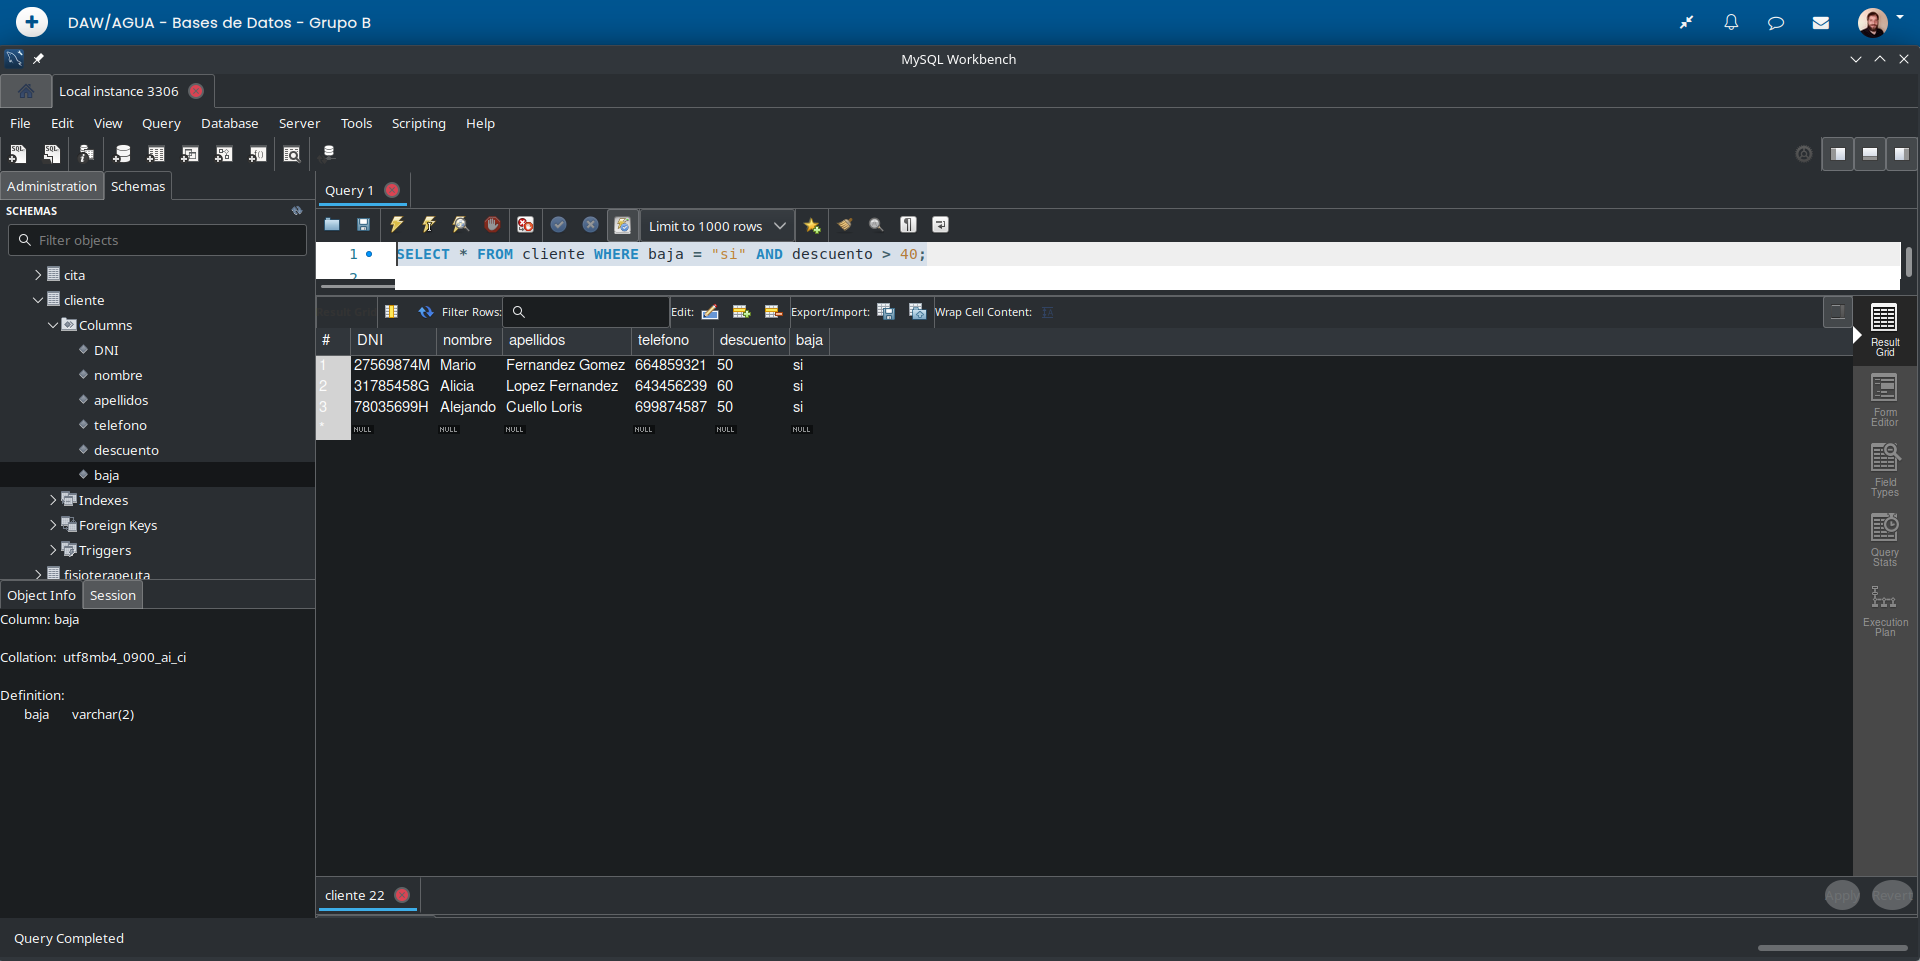
\includegraphics[scale=0.28]{resultado-consulta-4.png}
        \caption{Resultado Consulta nº 4}
    \end{figure}
\end{enumerate}

\subsection{Apartado B}



% Bibliography

%\newpage
%\bibliography{citas}
%\bibliographystyle{unsrt}

\end{document}